
\documentclass[aspectratio=169,xcolor=dvipsnames]{beamer}
%\usetheme{SimplePlus}

\usepackage{hyperref}
\usepackage{graphicx} % Allows including images
\usepackage{booktabs} % Allows the use of \toprule, \midrule and \bottomrule in tables

%----------------------------------------------------------------------------------------
%	TITLE PAGE
%----------------------------------------------------------------------------------------

\title[PLS]{Ladder Diagram (LD) programmering} % The short title appears at the bottom of every slide, the full title is only on the title page
%\subtitle{Subtitle}

\author[Fred-Olav] {Fred-Olav Mosdal}

\institute[Gand VGS] % Your institution as it will appear on the bottom of every slide, may be shorthand to save space
{
    Gand VGS \\
    VG3 Automasjon }
\date{\today} % Date, can be changed to a custom date


%----------------------------------------------------------------------------------------
%	PRESENTATION SLIDES
%----------------------------------------------------------------------------------------

\begin{document}
\begin{frame}
\titlepage
\end{frame}



\begin{frame}
	\frametitle{Eksempel på ladder program}
	$$\includegraphics[width=0.9\textwidth]{plc_022.eps}$$
\end{frame}

\begin{frame}
	\frametitle{Kontakter og spoler}
	\begin{columns}
		\begin{column}{0.5\textwidth}
	\begin{itemize}
		\item grunnleggende i LD, erstatter brytere og relespoler i relesyringer
	\end{itemize}
		\end{column}
		\begin{column}{0.5\textwidth}
	$$\includegraphics[width=1\textwidth]{plc_023.eps}$$
		\end{column}
	\end{columns}
\end{frame}















\end{document}
